
\documentclass[12pt]{article}
\usepackage{setspace}
\doublespacing
\usepackage{fullpage}
\usepackage{amsbsy}
\usepackage{amsmath}
\usepackage{amsfonts}
\usepackage{amsthm}
\usepackage{amssymb}
\usepackage{algorithmic}
\usepackage{algorithm}
\usepackage{enumerate}
\usepackage{epsfig}
\usepackage{graphicx}
\usepackage{multirow}
%\usepackage{natbib}
\usepackage{xr}
\usepackage{color}
\usepackage{subfigure}
\numberwithin{equation}{section}

%%%%%%%%%%%%%%%%%%%%%%%%%%%%%%%%%%%%%%%%%%%%%%%%%%%%%%%%%%

\begin{document}

\title{\bf{Matrix Multiplication \\ CS 5220: Homework 1}}

\author{Group 9 \\ Ze Jin (zj58)\quad Sam Tung (sat83) \quad Patrick Cao (pxc2) \\}

\date{ }
%\date{\today}

\maketitle





\section{Method}

We refer to the tuning ideas on the note ``Tuning on a single core''.

\subsection{Loop Order}

In the naive implementation, we loop over $i$, then $j$, then $k$.
\\
Alternative loop order might be more cache friendly. For example, using the $(i,j,k)$ order, we have to go across a row of $A$ in the inner loop, which is a non-unit-stride access.
\\
We compare different orders, including $(i,k,j), (j,i,k), (j,k,i)$.

\subsection{Blocking}

We can partition matrices into small blocks, and apply the block matrix multiplication.
\\
The advantage is that original matrices cannot fit into cache while the little blocks can.
\\
We compare different block sizes, including 2, 4, 8, 16, 32, 64, 128.

\subsection{Copy Optimization}

We might run into conflict misses associated with cache. One way to solve the problem is to explicitly copy blocks into a contiguous block of local storage before multiplying them.
\\
Another side benefit of copy optimization is that we can use it to gracefully deal with fringe blocks.
\\
Therefore, we add copy optimization to one-layer and two-layer blocking.
\\
In one-layer blocking with copy optimization, we compare different block sizes, including 2, 4, 8, 16, 32, 64, 128.
\\
In two-layer blocking with copy optimization, we compare different block size pairs, including (64,2), (64,4), (64,8), (64,16), (64,32), (128, 64), (256,64), (512,64).

\subsection{Compiler Flag}

It is worthwhile playing with the flags that control the compiler optimizations, since modern compilers do some types of optimizations much better than people do.
\\
We compile the code with option \texttt{-funroll-loops} to unroll loops (basic loop unrolling is automatic with -O3).

\section{Result}

We run jobs on the totient cluster, and get the results depicted in several plots.

\subsection{Loop Order}

See Figure 1, 2, 3 and 4 below for loop order.
\\
The plot shows that looping performs the best with loop order $(j, k, i)$.

\begin{figure}[!ht]
   \begin{subfigure}
      \centering
        \begin{center}
      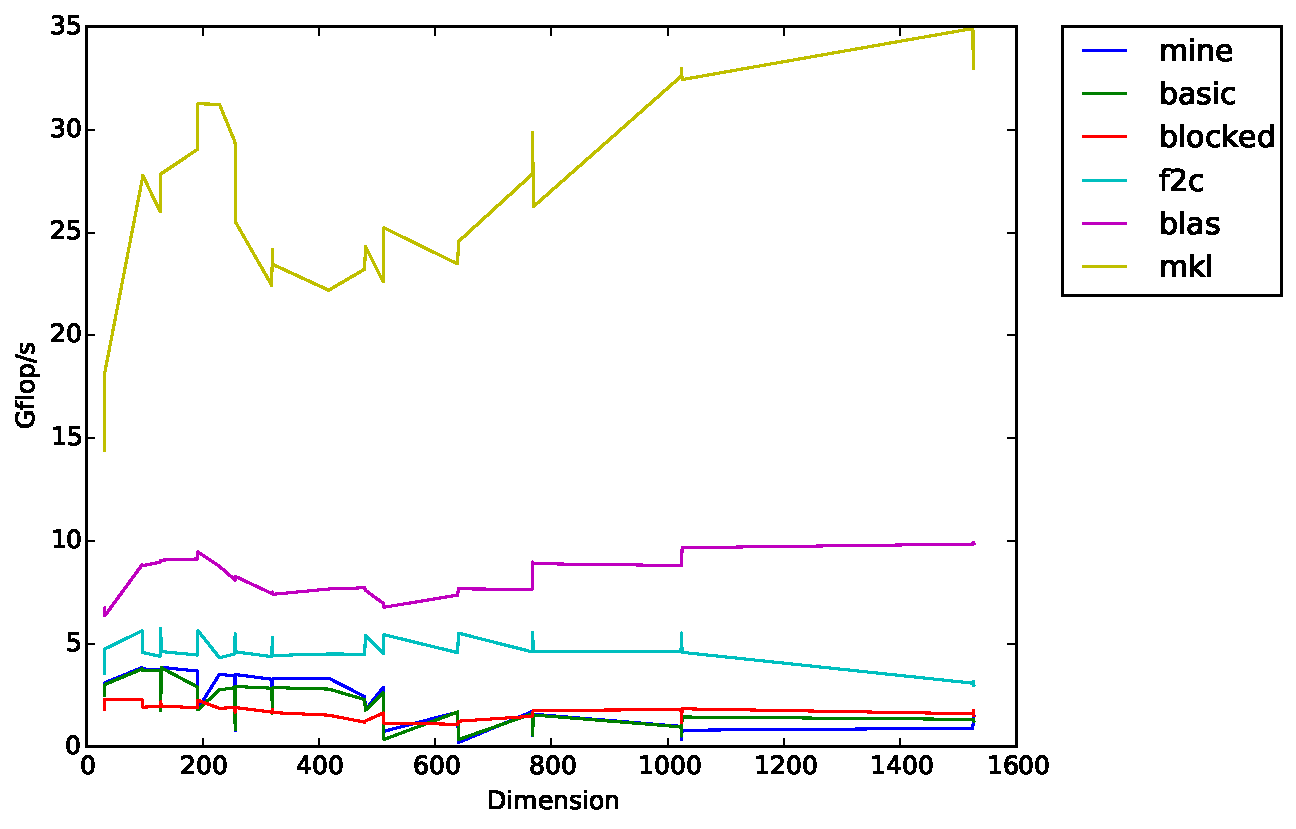
\includegraphics[width=0.85\textwidth] {ijk}
        \end{center}
      \label{aload0}
      \caption{loop order: $(i, j, k)$}
  \end{subfigure}
  \begin{subfigure}
      \centering
        \begin{center}
      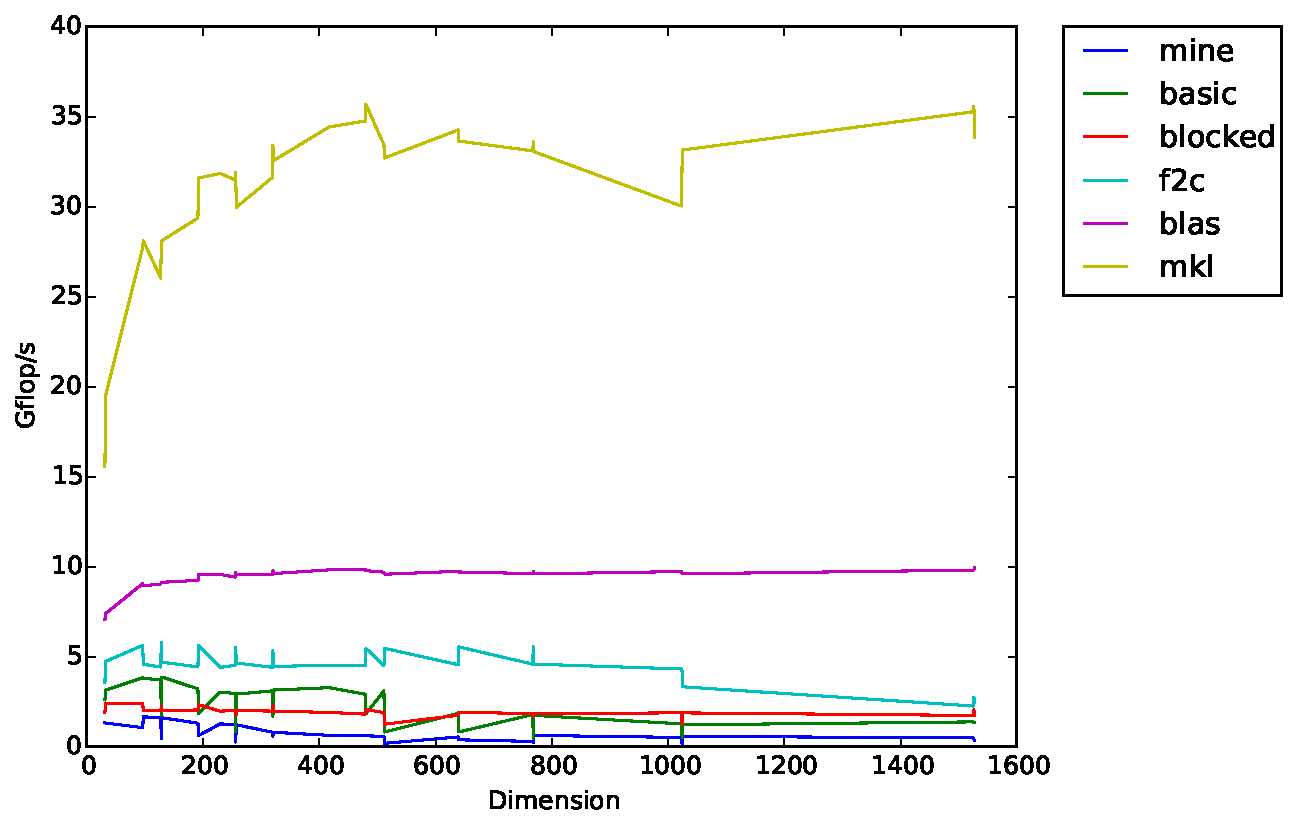
\includegraphics[width=0.85\textwidth] {ikj}
        \end{center}
      \label{aload1}
      \caption{loop order: $(i, k, j)$}
  \end{subfigure}

\end{figure}

\begin{figure}[!ht]
   \begin{subfigure}
      \centering
        \begin{center}
      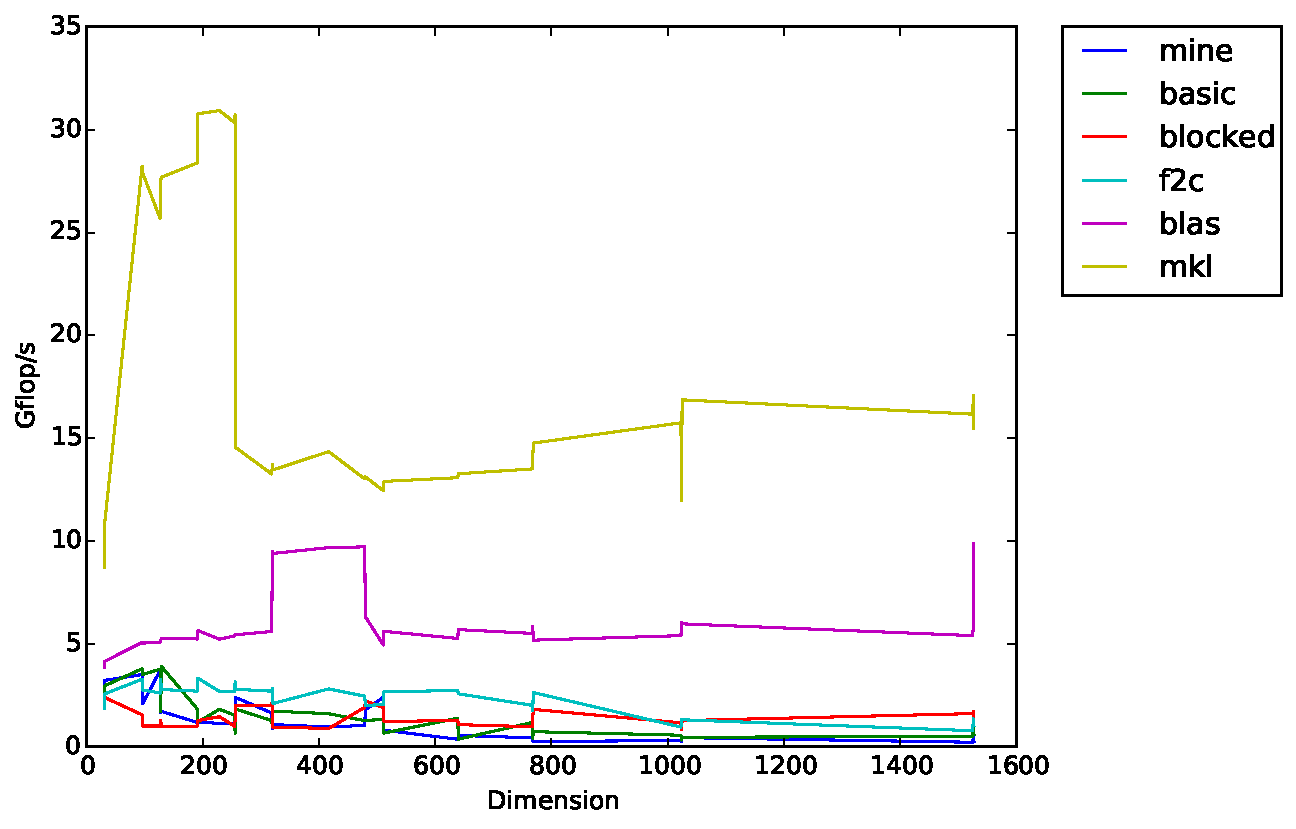
\includegraphics[width=0.85\textwidth] {jik}
        \end{center}
      \label{aload0}
      \caption{loop order: $(j, i, k)$}
  \end{subfigure}
  \begin{subfigure}
      \centering
        \begin{center}
      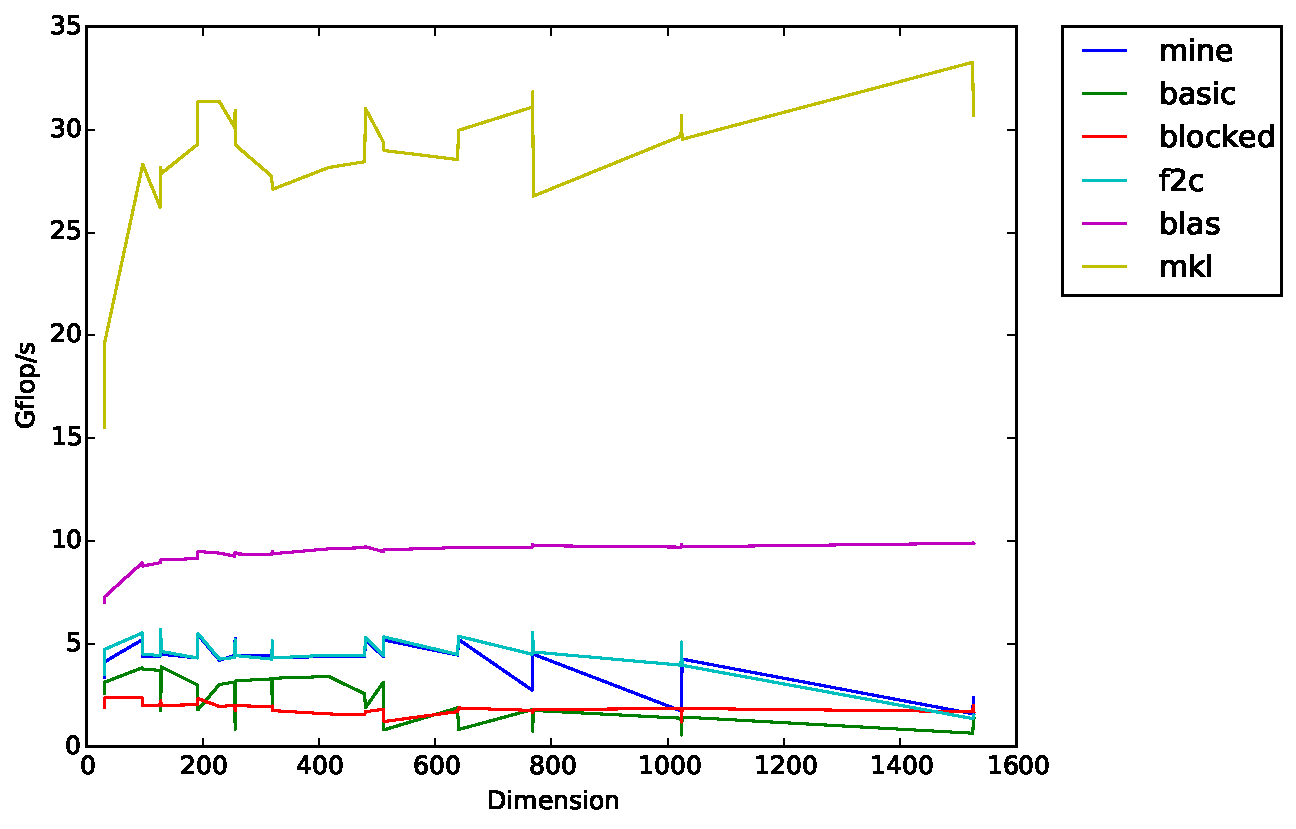
\includegraphics[width=0.85\textwidth] {jki}
        \end{center}
      \label{aload1}
      \caption{loop order: $(j, k, i)$}
  \end{subfigure}

\end{figure}

\subsection{Blocking}

See Figure 5 and 6 below for one-layer blocking.
\\
The plot shows that one-layer blocking performs the best with block size $= 64, 128, 256$.

\begin{figure}[!ht]
   \begin{subfigure}
      \centering
        \begin{center}
      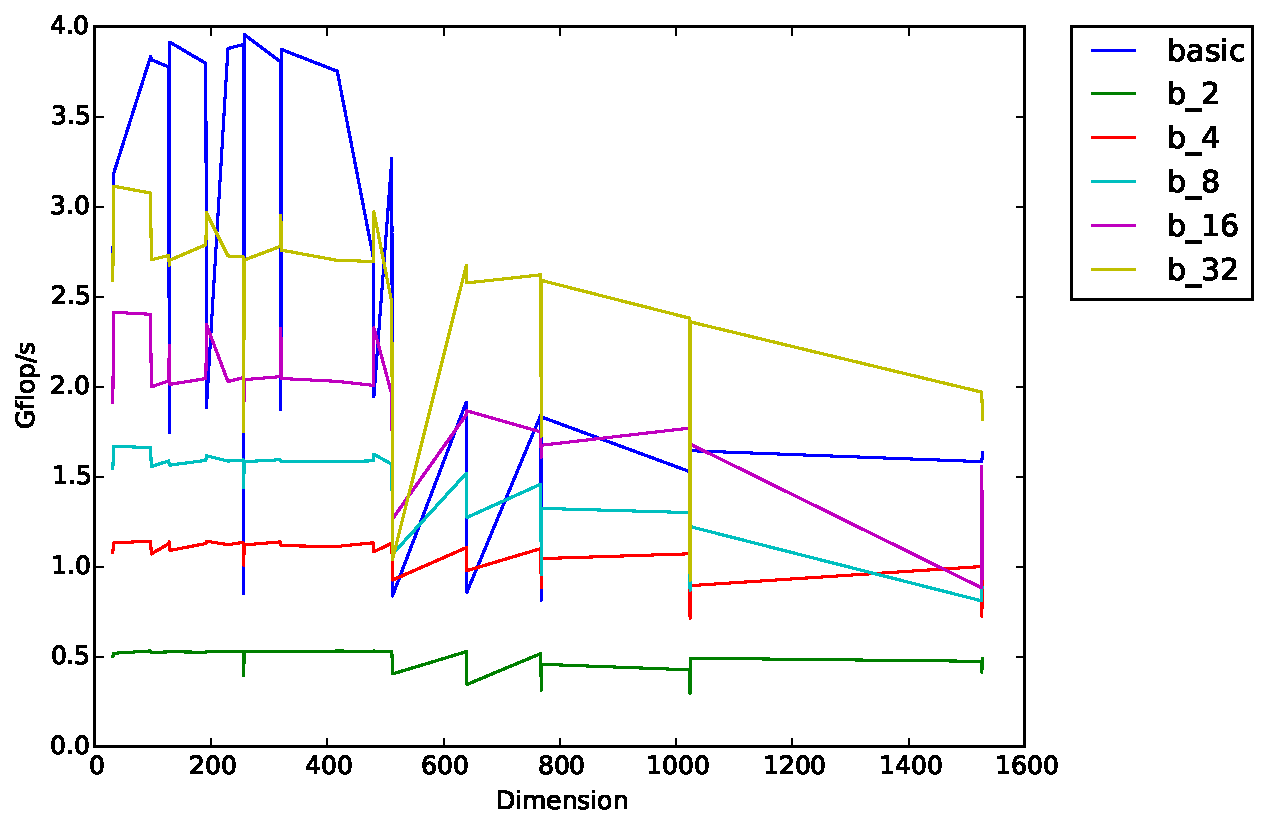
\includegraphics[width=0.85\textwidth] {timing_b_1}
        \end{center}
      \label{aload0}
      \caption{one layer of blocking}
  \end{subfigure}
  \begin{subfigure}
      \centering
        \begin{center}
      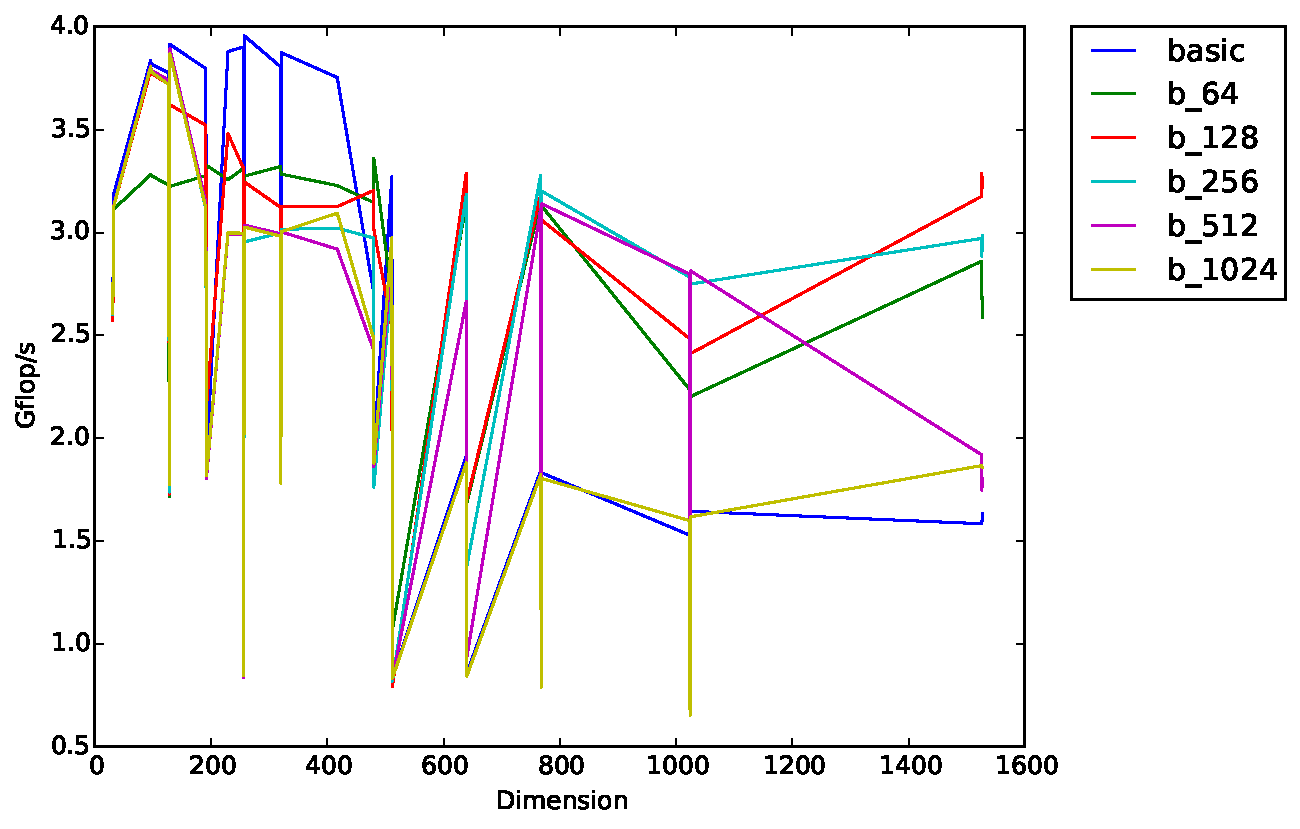
\includegraphics[width=0.85\textwidth] {timing_b_2}
        \end{center}
      \label{aload1}
      \caption{one layer of blocking}
  \end{subfigure}

\end{figure}

\subsection{Blocking and Copy Optimization}

See Figure 7 and 8 below for one-layer blocking with copy optimization.
\\
The plot shows that one-layer blocking with copy optimization performs the best with block size $= 32, 64$.
\\
See Figure 9 and 10 below for two-layer blocking with copy optimization.
\\
The plot shows that two-layer blocking with copy optimization performs the best with block size pair $= (64, 32), (128, 64), (256, 64), (512, 64)$.

\begin{figure}[!ht]
   \begin{subfigure}
      \centering
        \begin{center}
      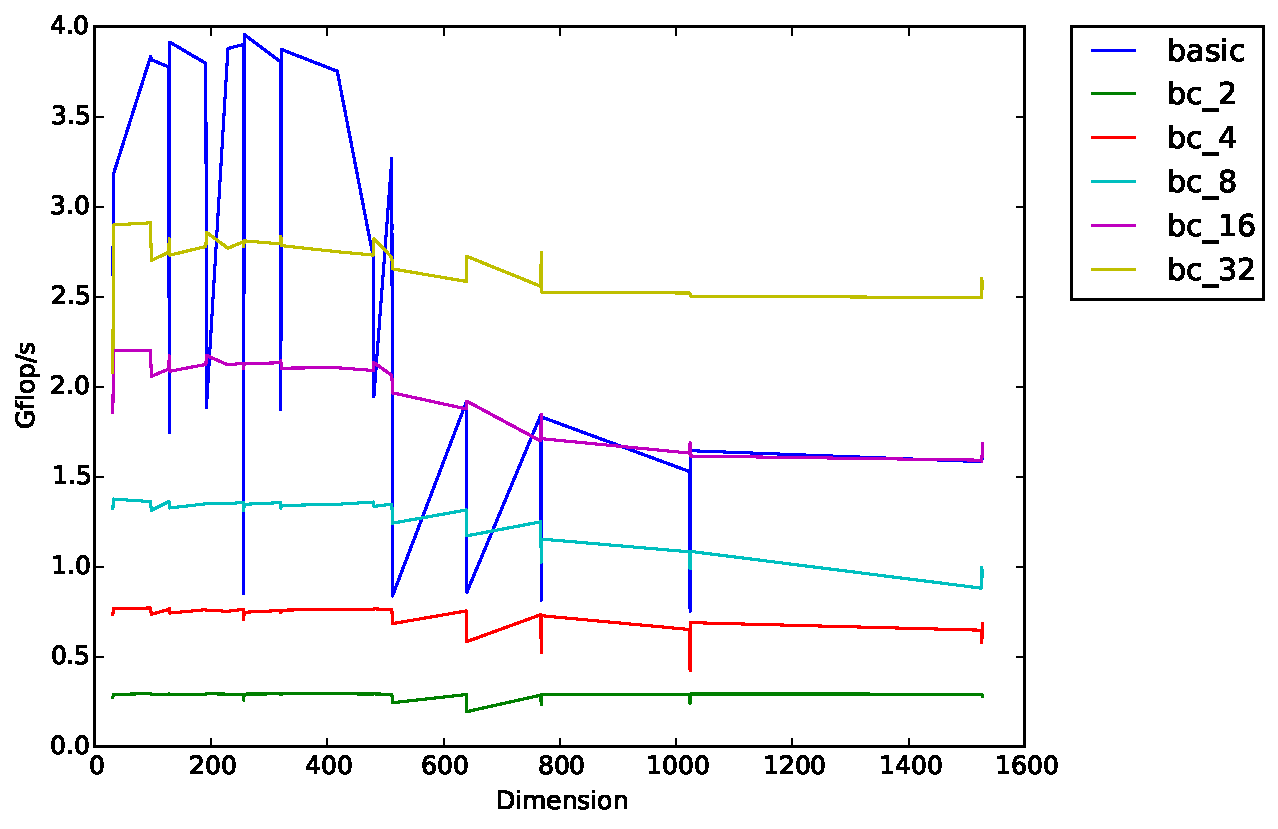
\includegraphics[width=0.85\textwidth] {timing_bc_1}
        \end{center}
      \label{aload0}
      \caption{one layer of blocking with copy optimization}
  \end{subfigure}
  \begin{subfigure}
      \centering
        \begin{center}
      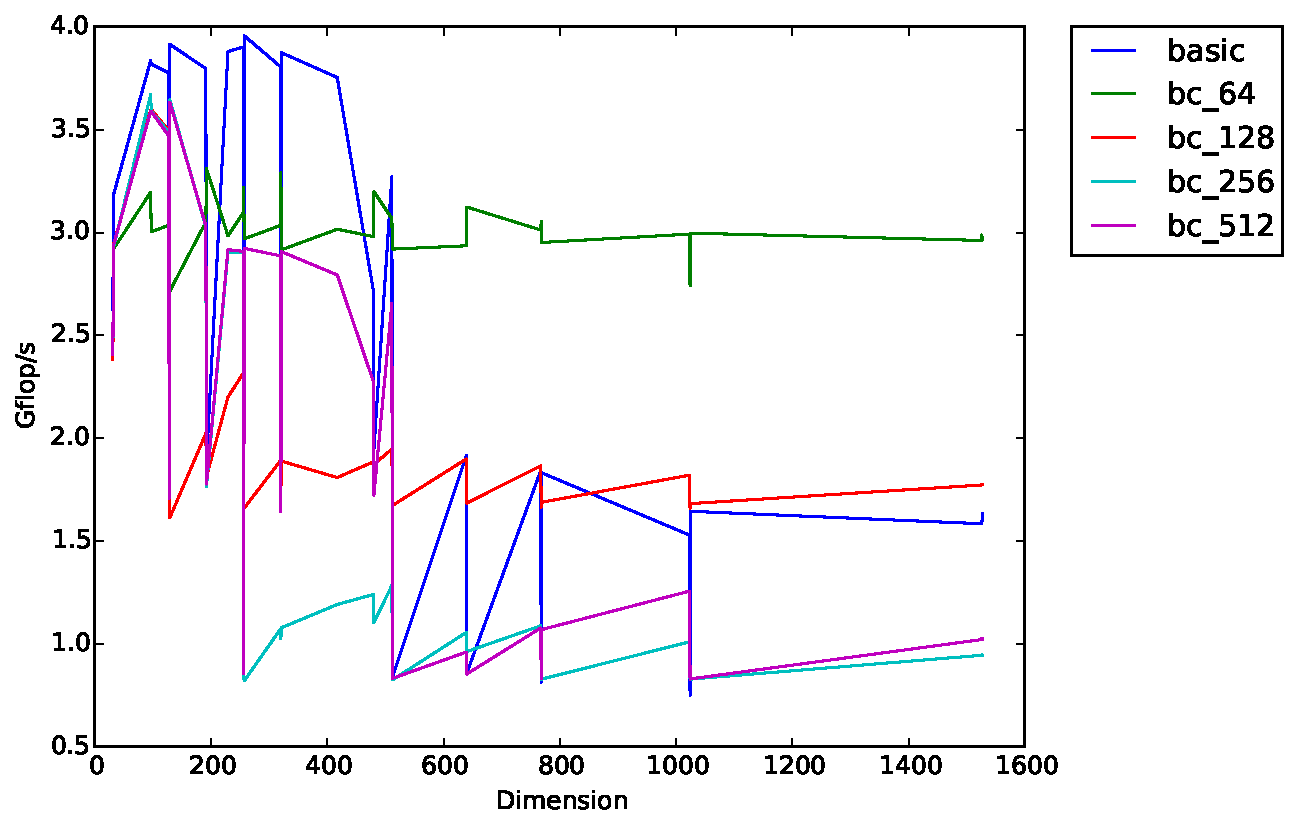
\includegraphics[width=0.85\textwidth] {timing_bc_2}
        \end{center}
      \label{aload1}
      \caption{one layer of blocking with copy optimization}
  \end{subfigure}

\end{figure}

\begin{figure}[!ht]
   \begin{subfigure}
      \centering
        \begin{center}
      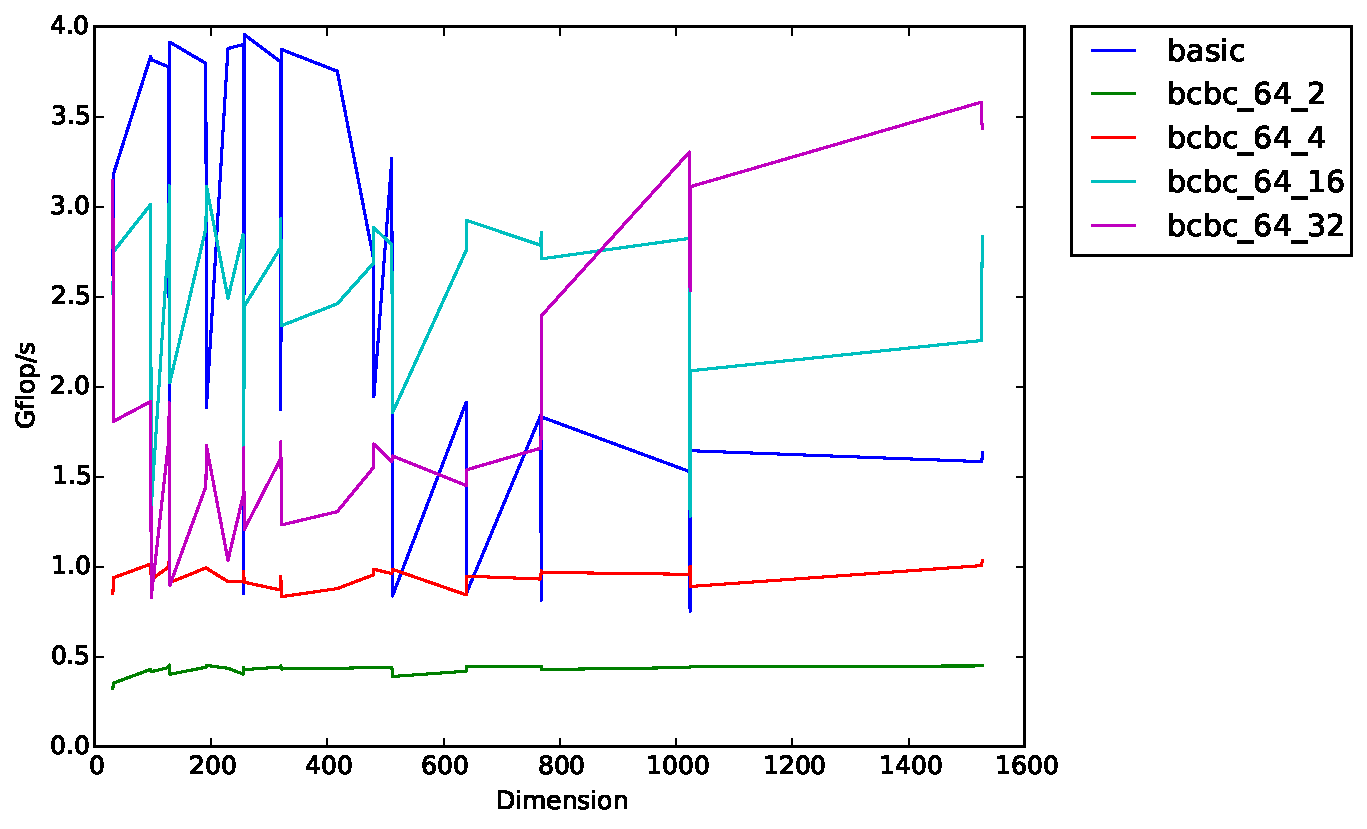
\includegraphics[width=0.85\textwidth] {timing_bcbc_1}
        \end{center}
      \label{aload0}
      \caption{two layers of blocking with copy optimization}
  \end{subfigure}
  \begin{subfigure}
      \centering
        \begin{center}
      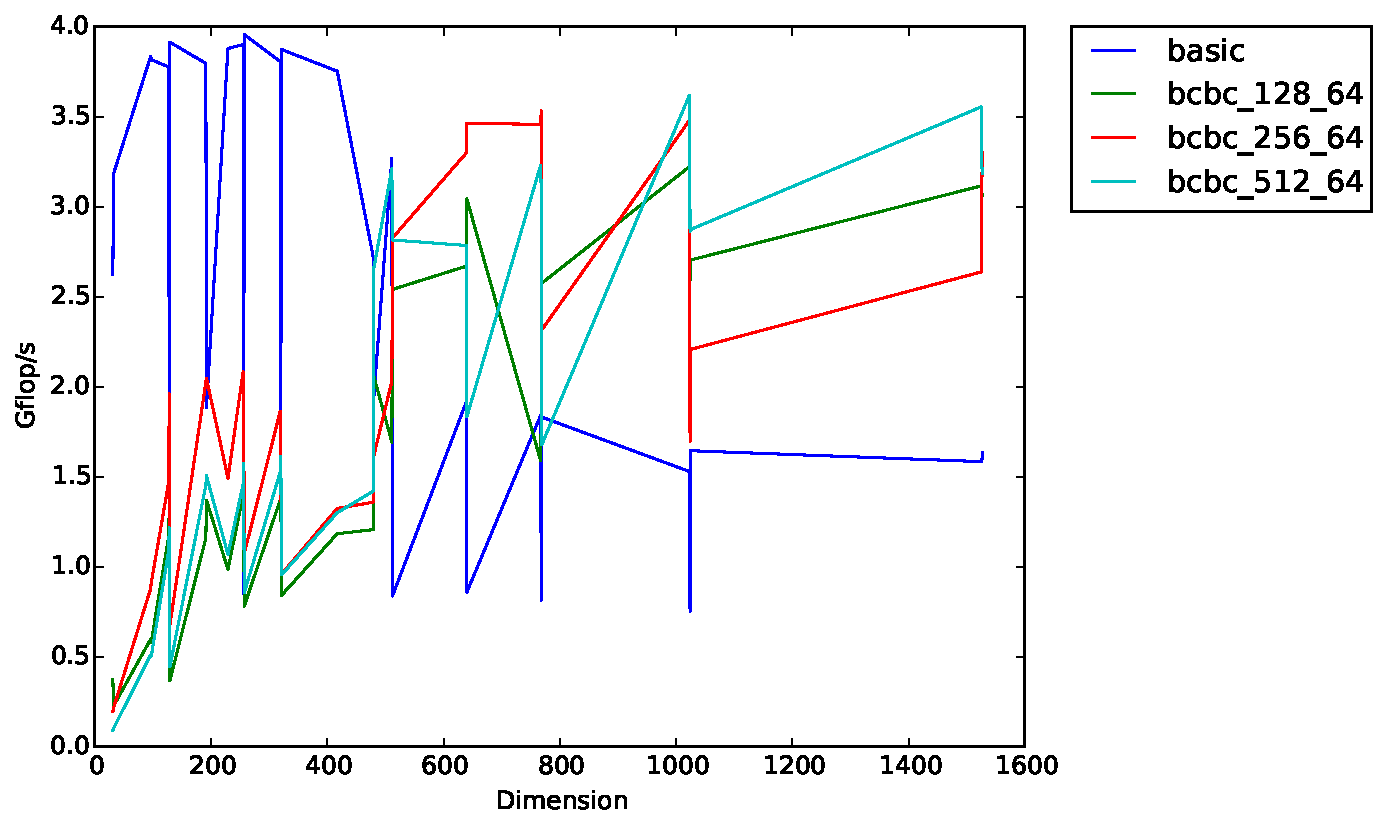
\includegraphics[width=0.85\textwidth] {timing_bcbc_2}
        \end{center}
      \label{aload1}
      \caption{two layers of blocking with copy optimization}
  \end{subfigure}

\end{figure}

\subsection{Compiler Flag}

See Figure 11 below for unrolling loops in compiler flags.
\\
The plot shows that unrolling loops in compiler flags alone does not make much difference.

\begin{figure}[!ht]
\begin{center}
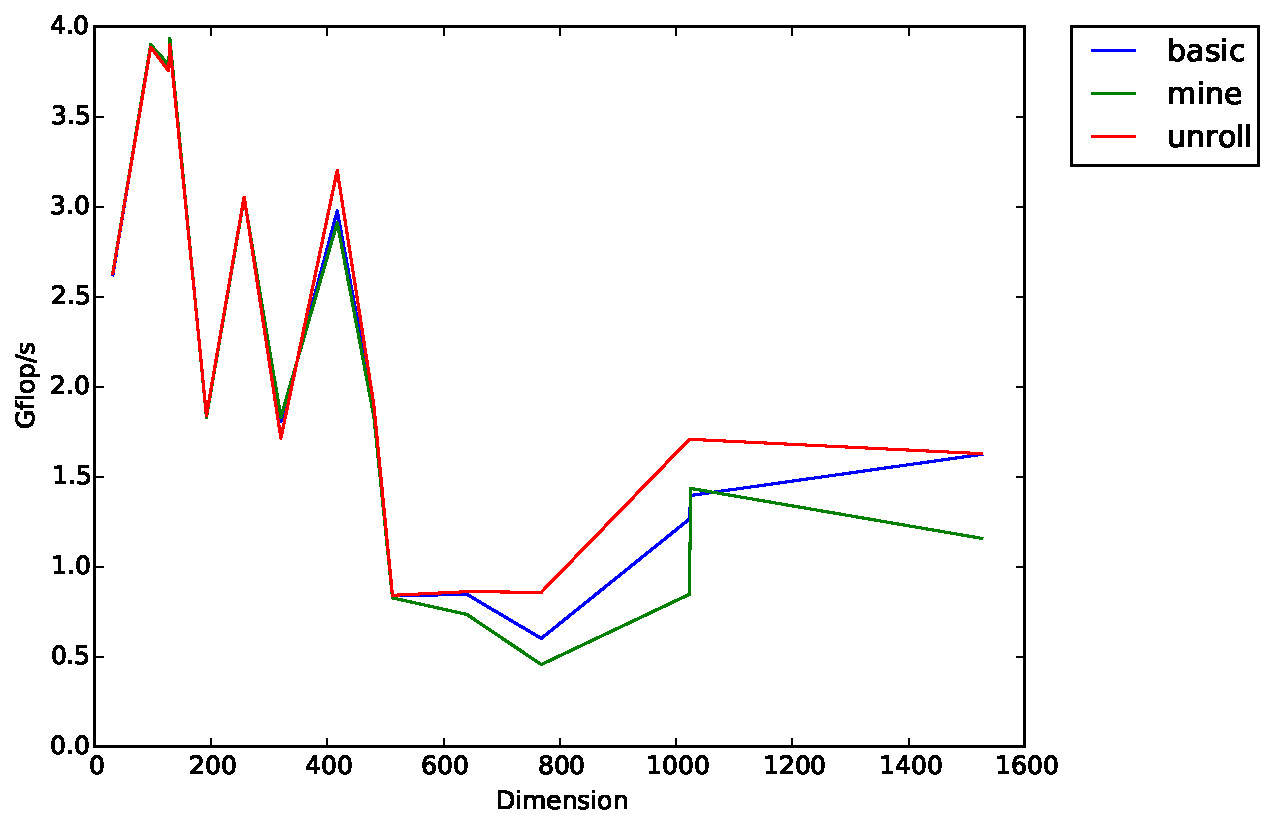
\includegraphics[width=0.85\textwidth] {timing_unroll}
\caption{unrolling loops in compiler flags}
\end{center}
\end{figure}





\section*{Reference}

(1) David Bindel, Tuning on a single core, Applications of Parallel Computers (CS 5220), Fall 2011.



\end{document}





